
\begin{frame}[noframenumbering,plain]
    \mytitle{Contributions}
    \vspace{1cm}

    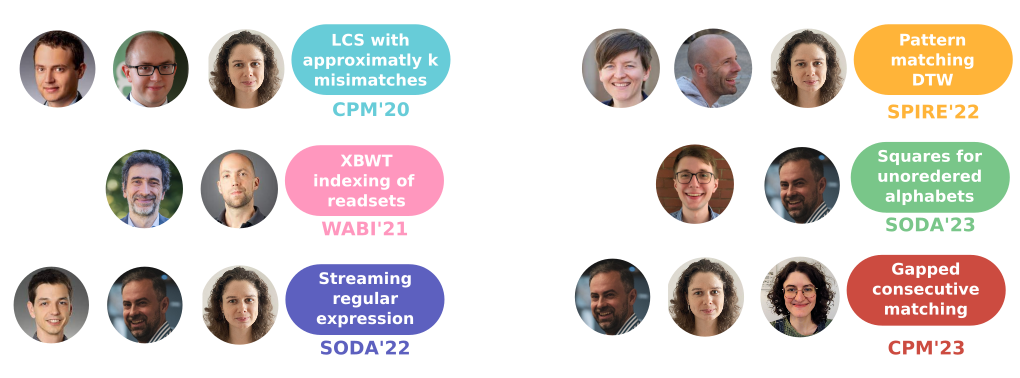
\includegraphics[width=\textwidth]{pictures/mindmap/co_auth.png}
\end{frame}

\begin{frame}[noframenumbering,plain]
    \only<1|handout:0>{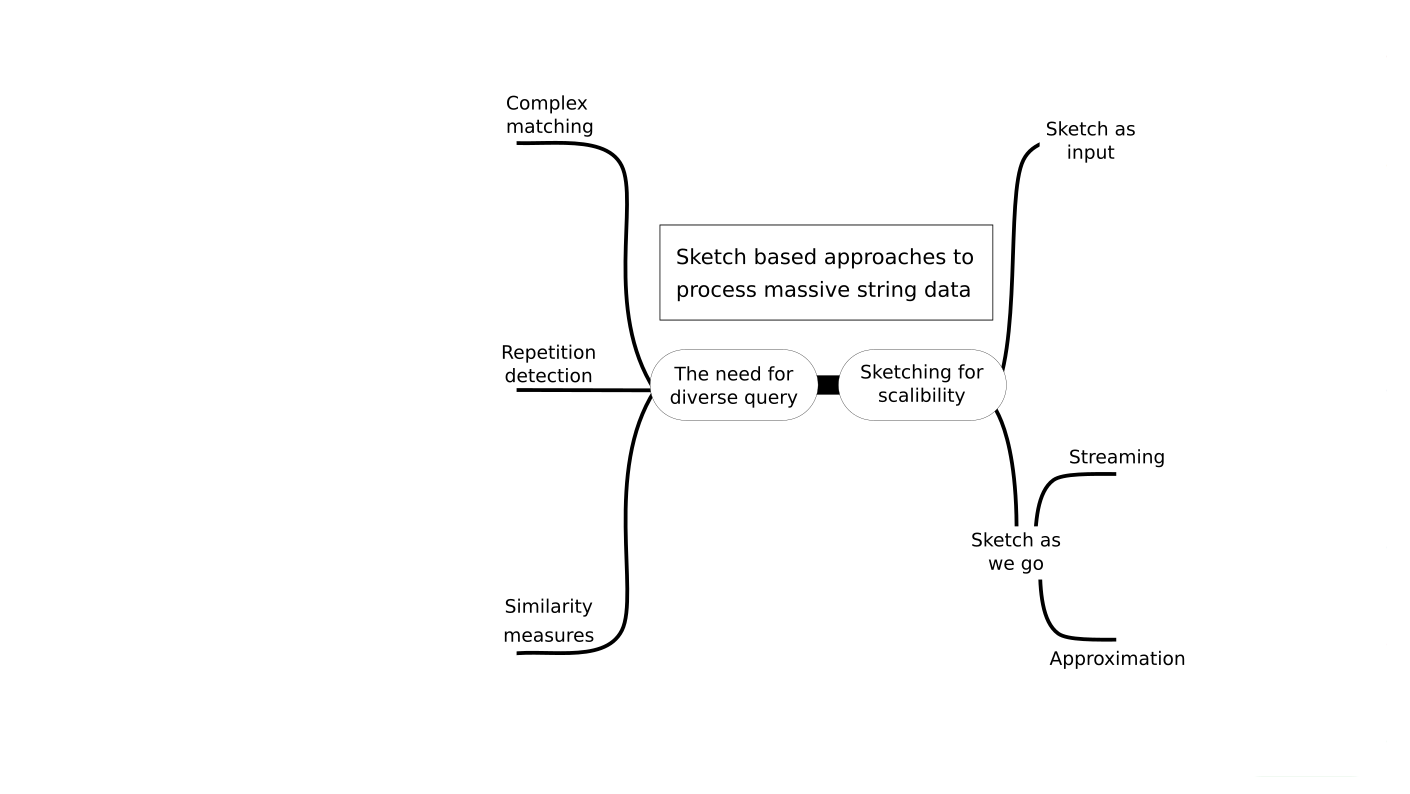
\includegraphics[width=\textwidth]{pictures/mindmap/3.png}}
    \only<2|handout:0>{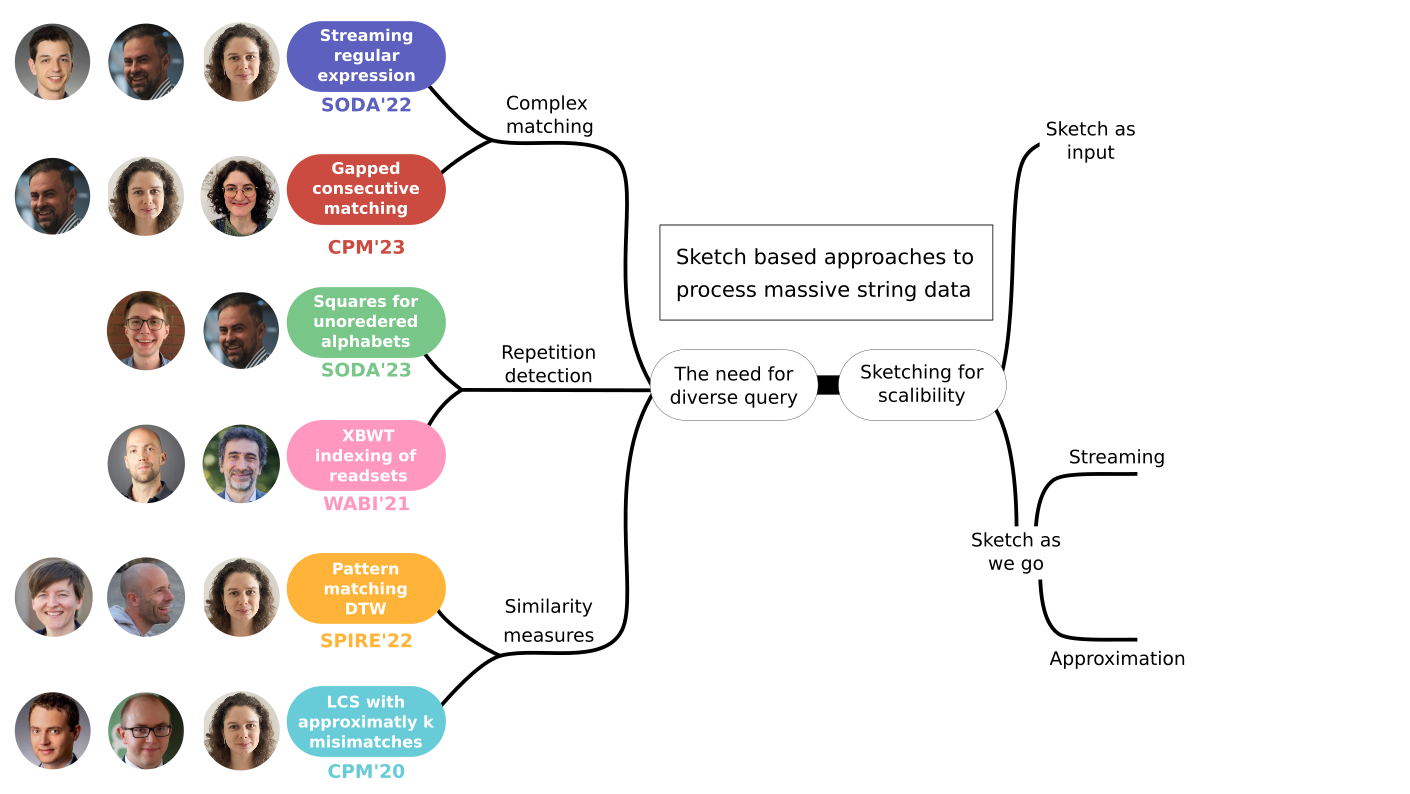
\includegraphics[width=\textwidth]{pictures/mindmap/4.png}}
    \only<3|handout:0>{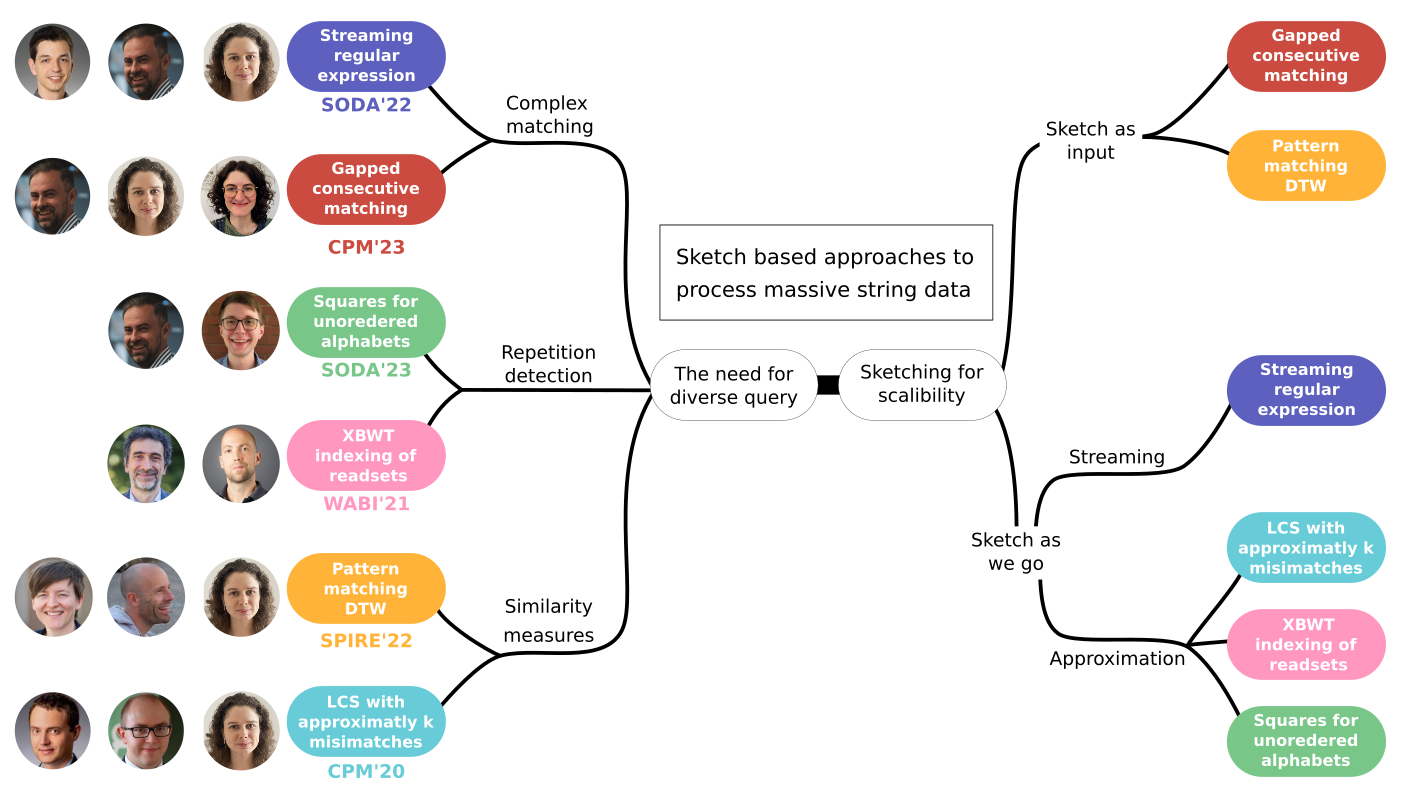
\includegraphics[width=\textwidth]{pictures/mindmap/5.png}}
    \only<4>{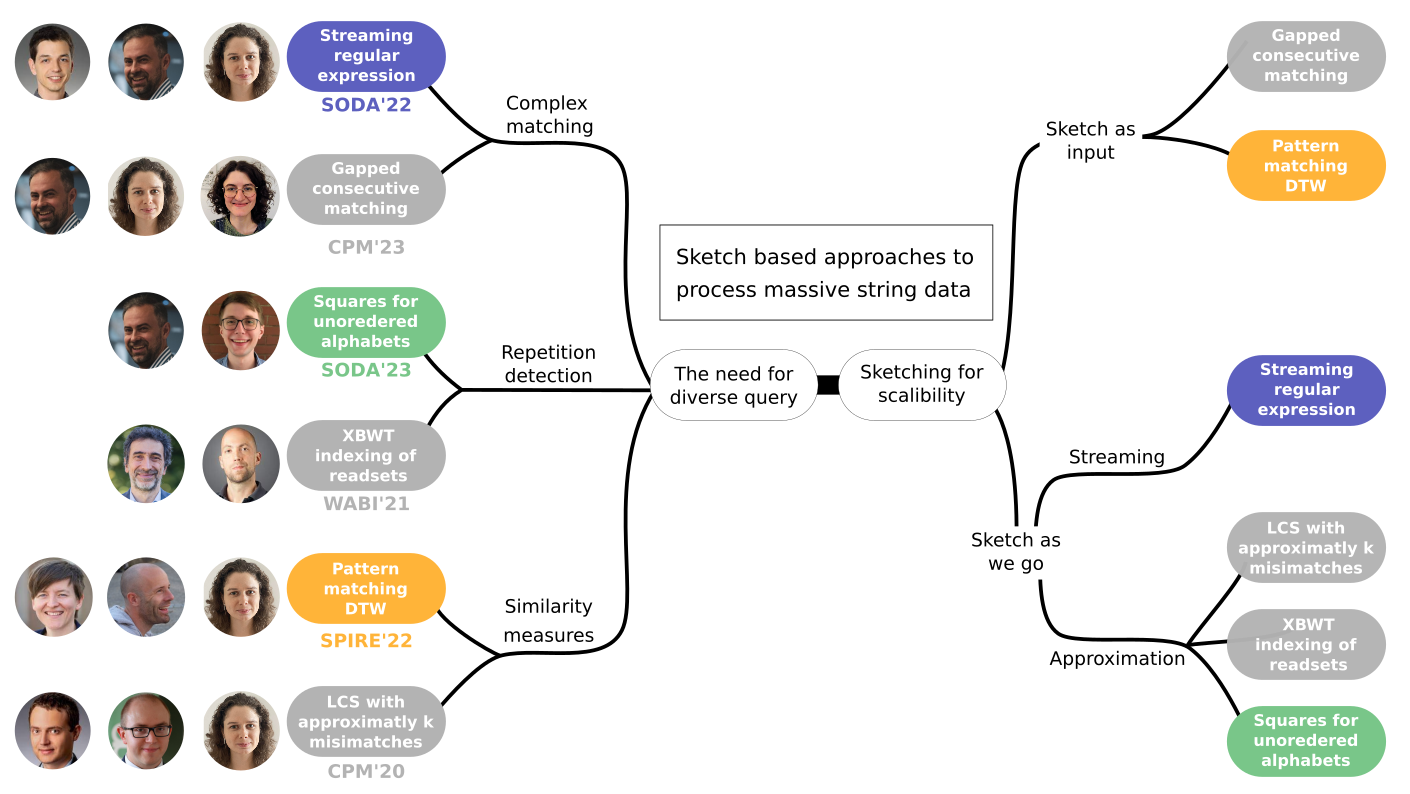
\includegraphics[width=\textwidth]{pictures/mindmap/present.png}}
\end{frame}

\begin{frame}
    
\includegraphics[width=\textwidth]{pictures/mindmap/regexp.png}
\end{frame}

\begin{frame}{A powerful matching model: regular expressions}
    \begin{columns}
        \column{.6\textwidth}
        \begin{mydefblock}{Regular expressions}
            either a character from $\Sigma$ or recursively defined from other regular expressions $R_1$ and $R_2$:
            \pause
            \begin{enumerate}
                \item $R_1 \cdot R_2$ (concatenation),
                \pause
                \item $R_1 | R_2$ (union),
                \pause
                \item $R_1^\ast$ (Kleene star).
            \end{enumerate}
            \pause
        \end{mydefblock}
        \column{.4\textwidth}
        \begin{center}
            \only<1|handout:0>{\textbf{Ex:} For $\Sigma=\{a,b\}$,\\ 
             $R_1=a$ only matches $a$,\\
             and $R_2=b$ only matches $b$.}
            \only<2|handout:0>{$R_1 \cdot R_2$ matches anything matching $R_1$ followed by anything matching $R_2$.\\
            \textbf{Ex:} with $R_1=a$ and $R_2=b$, $R_1 \cdot R_2$ matches $ab$.}
            \only<3|handout:0>{$R_1 | R_2$ matches anything matching $R_1$ or  $R_2$.\\
            \textbf{Ex:} with $R_1=a \cdot b = ab$ and $R_2=b$, $R_1 \cdot R_2$ matches $ab$ and $b$.}
            \only<4|handout:0>{$R_1^\ast$ matches any number of repetition of any string matching $R_1$.\\
            \textbf{Ex:} with $R_1=(b|ab)$ matches $\varepsilon$, $ab$, $b$, $bbabb$...}
            \only<5->{
                \textbf{Ex:} $b(b|ab)^\ast ab$\\
                \smallskip
                \cmark ~ $bbbbbabab$ \\
                \cmark ~ $bbbabbbbab$\\
                \xmark ~ $bbbaabbbab$\\
                \xmark ~ $baba$\\ 
                \xmark ~ $abab$\\
                }
        \end{center}
    \end{columns}    
    \pause
    \pause

    \bigskip
    \only<7->{Used in databases, \pause data mining, \pause secret detection,\pause computer networks, \pause protein search\pause ...\\}
    \pause
    \bigskip
    \only<12->{
        \beamermathcolor{myblue}
        Given a regular expression $R$ and a text $T$, two problems:\\
        \bblue{Membership:} check if $R$ matches $T$.\\
        \bblue{Pattern matching:} check if $R$ matches \textbf{some substring} of $T$. \pause \textcolor{myblue}{Reduces to membership!}
    }
\end{frame}

\begin{frame}{A frugal model of computation: streaming}
\begin{columns}
    \column{.4\textwidth}
    The algorithm first receives and preprocesses the expression.\\ Next, it keeps reading characters from a very very long text and:
    \column{.5\textwidth}
    \begin{center}
        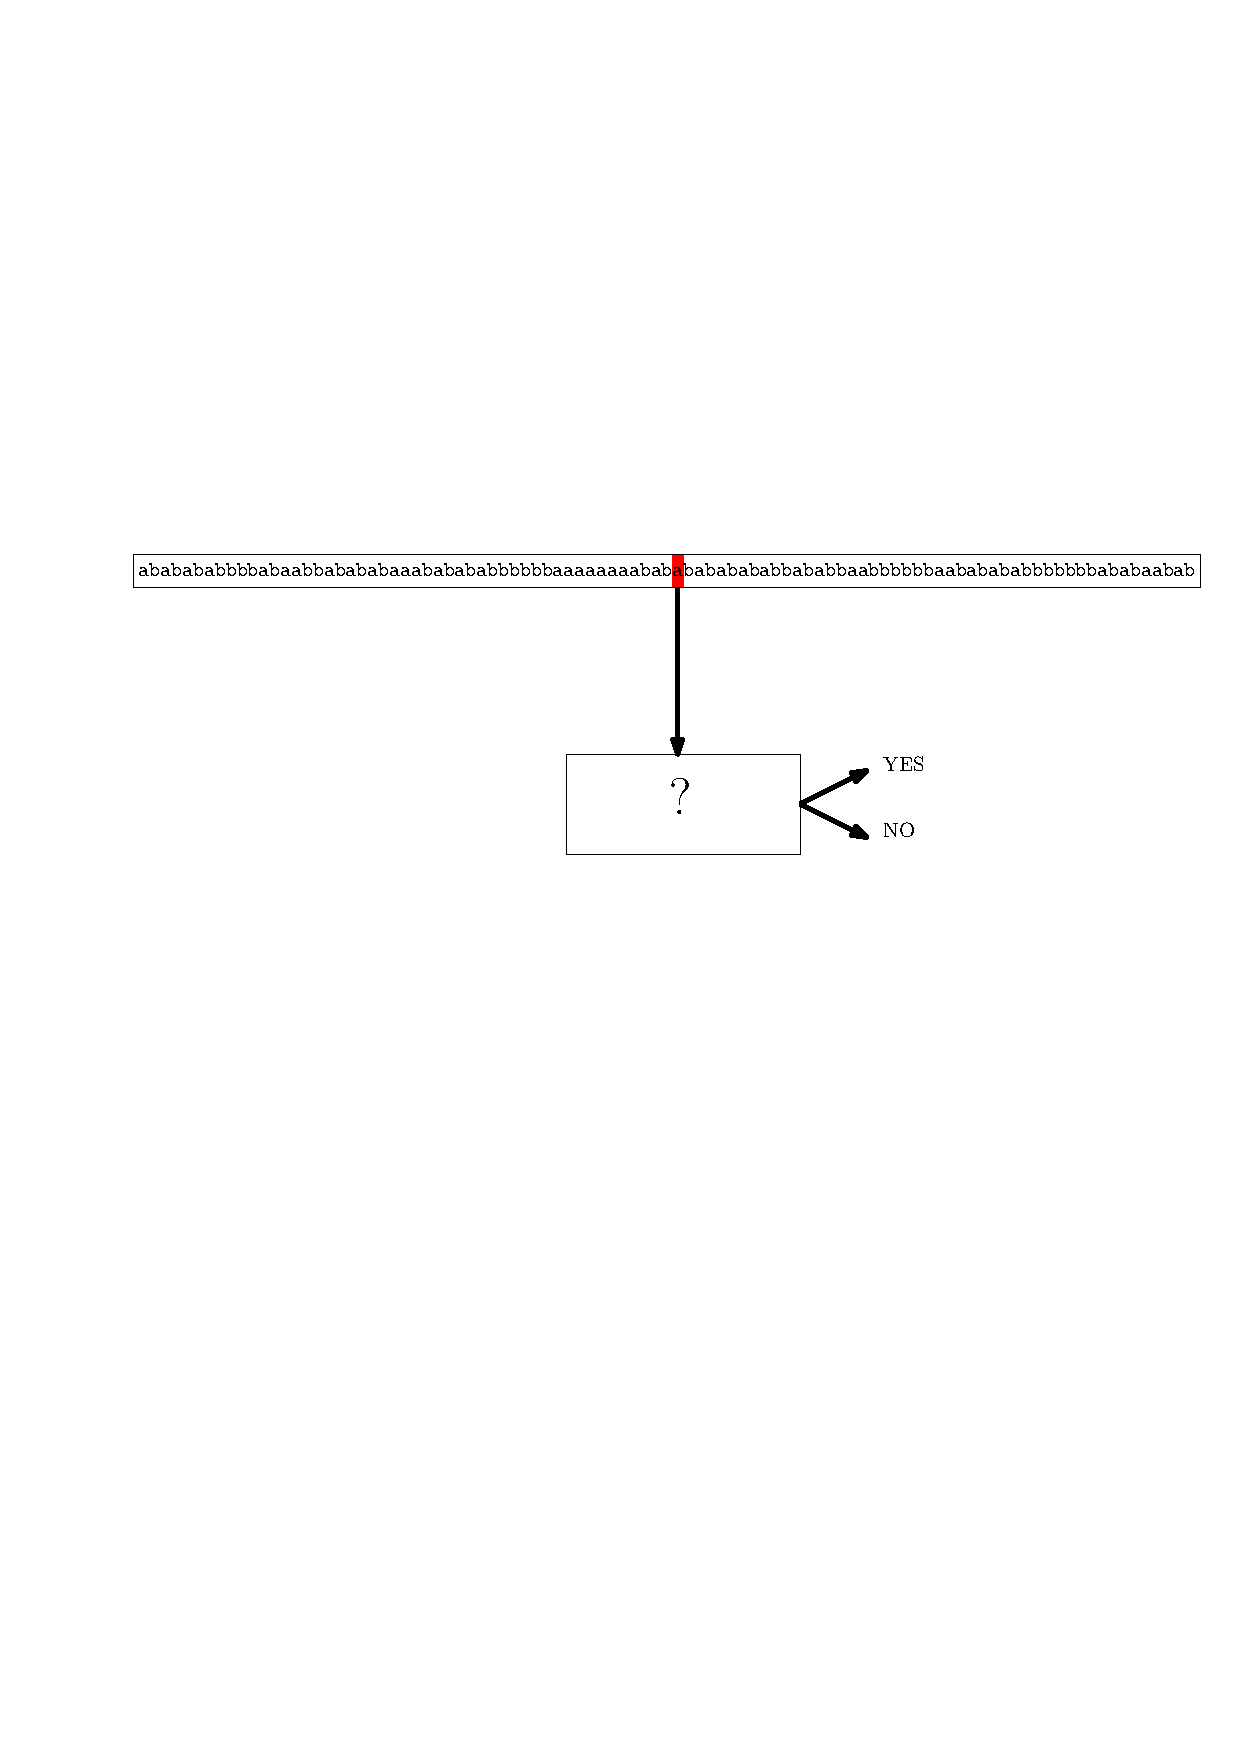
\includegraphics[width=\textwidth]{pictures/stream3}
    \end{center}
\end{columns}

\smallskip
\pause
\begin{enumerate}
\item No delay: After having seen the $i$-th character, immediately report whether the string so far matches the regular expression.
\pause
\item No going back: Not possible to read any of the earlier characters.
\pause
\item Every space counts: No access to the original expression (unless stored explicitly).
\end{enumerate}
\pause
\begin{mylemblock}{Classic pattern matching in streaming [Breslauer and Galil, TALG'14]}
    For a pattern of length $m$, it takes $\Oh(\log m)$ space and $\Oh(1)$ time per position.
\end{mylemblock}\pause
\begin{center}
    \small
    It relies on a variant of the Karp--Rabin fingerprints introduced by \ntheme{[Porat and Porat, FOCS'09]}.
\end{center}
\end{frame}

\begin{frame}{What can we do for regular expression membership in streaming ?}
    \begin{columns}
        \column{.35\textwidth}
        \ntheme{Classic:} Recursively build the \btheme{Thompson automata}, then check if $T$ is accepted.\\
        $\Oh(m)$ space and time/character.
        \column{.5\textwidth}
        \centering
        \begin{picture}(200,65)
            \put(0,0){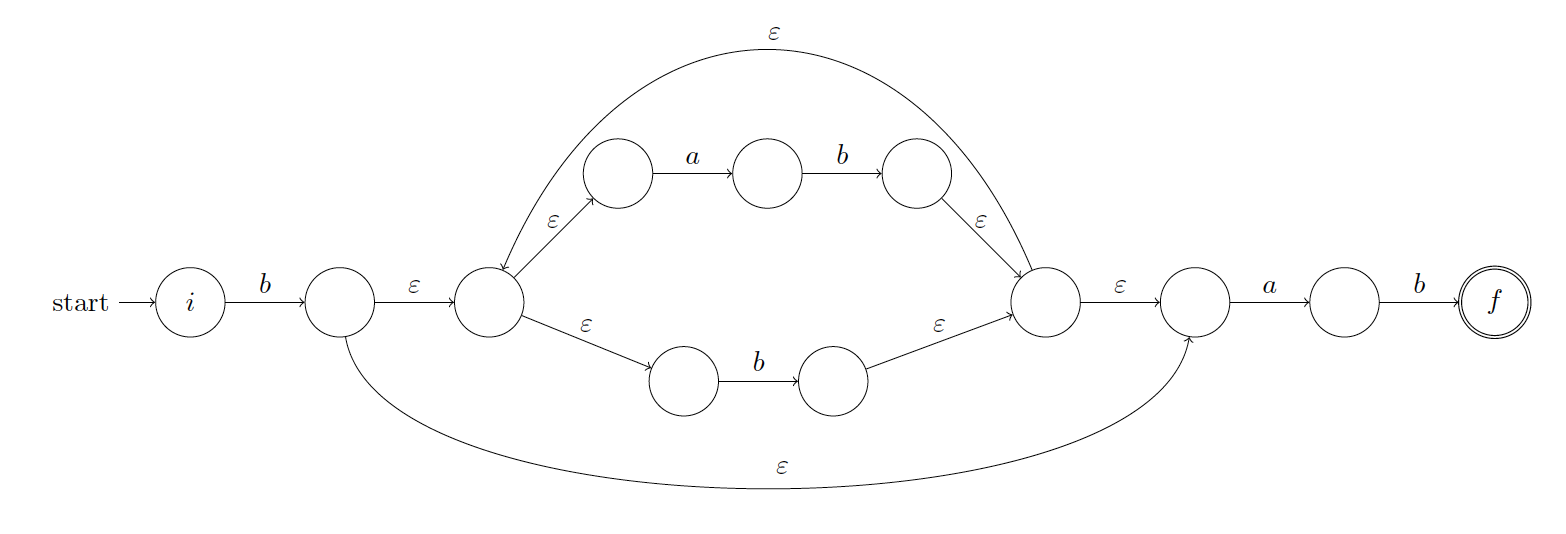
\includegraphics[width=\textwidth]{pictures/thomson1.png}}
            \put(150,50){\small $b(b|ab)^\ast ab$}
        \end{picture}
    \end{columns}
    \pause
    \begin{itemize}
        \item The best improvements on the time complexity \ntheme{only reduce by logarithmic factors}.\pause
        \item Fine-grained complexity showed that for \ntheme{``hard to match'' expressions we cannot do better}.\pause
        \item \ntheme{[Bille and Thorup, SODA'10]} Streaming time $\Oh(n\cdot (\frac{d\log w}{w}+\log d))$ and $\Oh(m)$ space, where $d$ is the number of occurrences of $|$ and $\ast$.\pause
        \item What about \btheme{space efficiency} ?\pause
    \end{itemize}
\end{frame}

\begin{frame}{What parameter is important for space-efficiency of regexp in Streaming ?}
    TODO: Dictionary and wildcards matching 

    \begin{myalertblock}{Dudek, Gawrychowski, Gourdel, Starikovskaya, SODA'22}
        For any regular expression $R$ with $d$ occurrences of $|$ and $\ast$, we can solve regular expression membership using $\Oh(d^{3}\polylog n)$ space and $\Oh(nd^{5}\polylog n)$ time per character.
    \end{myalertblock}
\end{frame}

\begin{frame}{}

    \begin{myalertblock}{Dudek, Gawrychowski, Gourdel, Starikovskaya, SODA'22}
        For any regular expression $R$ with $d$ occurrences of $|$ and $\ast$, we can solve regular expression membership using $\Oh(d^{3}\polylog n)$ space and $\Oh(nd^{5}\polylog n)$ time per character.
    \end{myalertblock}
    TODO: Intuition of how it works  
\end{frame}

\begin{frame}
    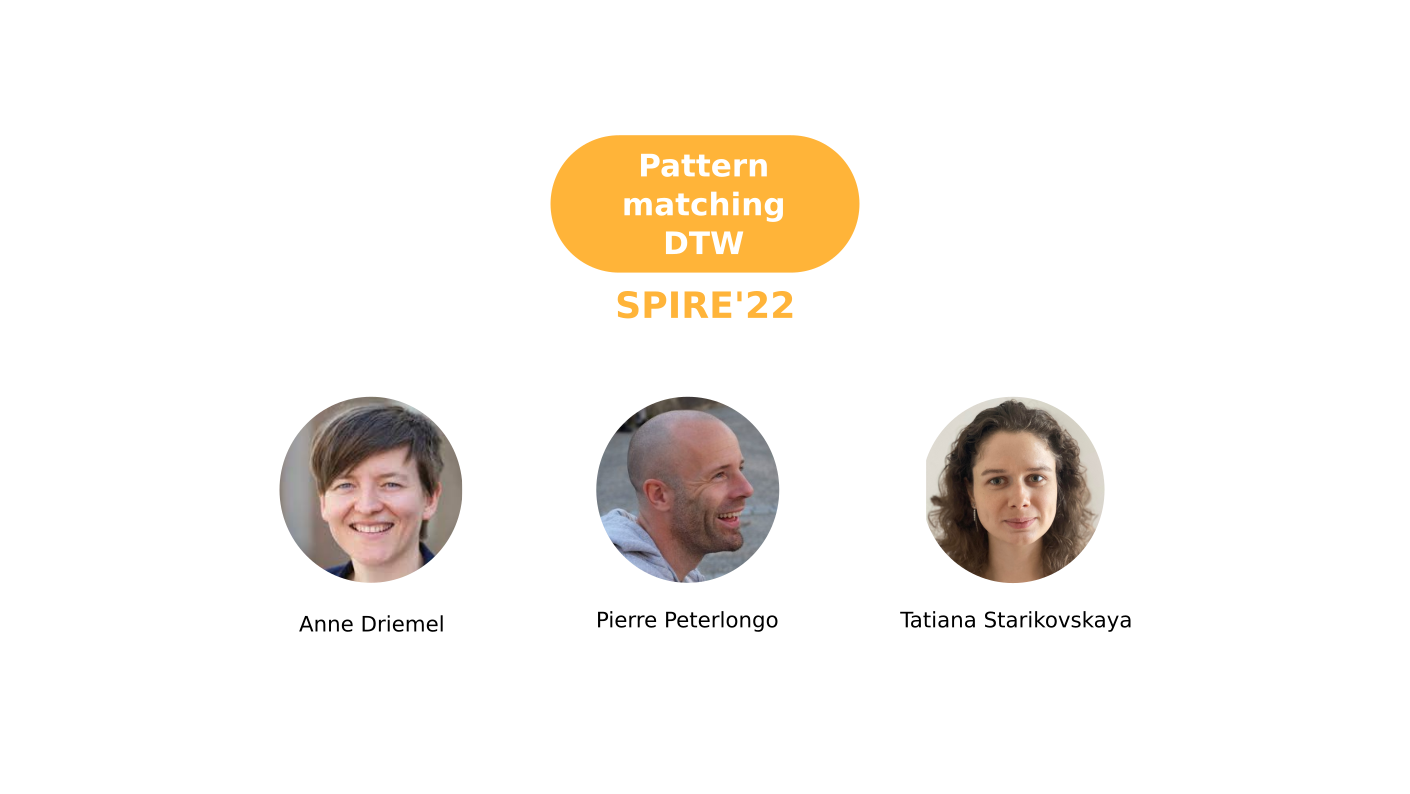
\includegraphics[width=\textwidth]{pictures/mindmap/dtw.png}
\end{frame}


\newcommand{\dtw}{\mathrm{DTW}}
\newcommand{\RLE}{\mathrm{RLE}}

\begin{frame}{Dynamic time warping (DTW) distance }

A \ntheme{measure of similarity between two temporal sequences} which can vary in speed.

\begin{center}
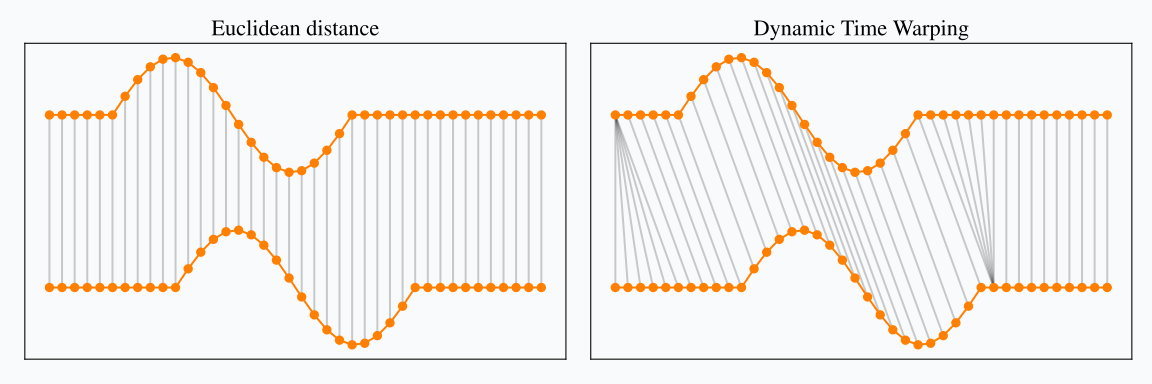
\includegraphics[scale=0.3]{figures/dtw_vs_euc.png}\footnote{Figure credit: Romain Tavenard}
\end{center}
\pause
Used in speech recognition to deal with varying speaking speeds.\pause

It has been studied for \ntheme{parametrized curves} where each item is a multidimensional point.

We focus on the setting where element are from a finite alphabet $\Sigma$, the sequences are \ntheme{strings}.

\end{frame}

\begin{frame}{Formal definition of $\dtw(X,Y)$}
\newcommand{\dtwgrid}[2]{% height width 
\foreach \i in {0,...,#1} {
	\foreach \j in {0,...,#2} {
		\filldraw[black] (\i , \j) circle (2pt);
		\ifthenelse{ \not \equal{#2}{\j}}{ 
			\draw[->] ($(\i , \j+0.9)$) -- ($(\i , \j+0.1)$);
		}{}
		\ifthenelse{ \not \equal{#1}{\i}}{
  			\draw[->] ($(\i +0.1 , \j)$) -- ($(\i +0.9 , \j)$);
		}{}
		\ifthenelse{\not\equal{#1}{\i} \and \not \equal{#2}{\j}}{%
  			\draw[->] ($(\i +0.1 , \j + 0.9)$) -- ($(\i +0.9, \j + 0.1)$);
  		}{}
	}
}
}

\newcommand{\dtwarrow}[2]{%
\draw[->,line width=0.3mm,red] #1 -- #2;
}

\begin{figure}
    \beamermathcolor{black}
    \centering
    \begin{tikzpicture}[scale=1, every node/.style={scale=1.5}]
    \dtwgrid{5}{2}

    \foreach \i in {1,...,6} {
        \node at ($(\i-1, 2.8)$) {\tiny{$X[\i]$}};
    }
    \foreach \j in {1,...,3} {
        \node at ($(-1.2, 3 -\j )$) {\tiny{$Y[\j]$}};
    }

    \foreach \x[count=\i] in {C,A,A,A,G,G} {
        \node at ($(\i-1 , 2.3)$) {\textcolor{black}{\tiny{\x}}};
    }
    \foreach \y[count=\j] in {A,T,G} {
        \node at ($(-0.5, 3 -\j )$) {\textcolor{black}{\tiny{\y}}};
    }


    \only<2->{
        \dtwarrow{(0.1,2)}{(0.9,2)}
        \dtwarrow{(3.1,1.9)}{(3.9,1.1)}
        \dtwarrow{(1.1,2)}{(1.9,2)}
        \dtwarrow{(2.1,2)}{(2.9,2)}
        \dtwarrow{(4,0.9)}{(4,0.1)}
        \dtwarrow{(4.1,0)}{(4.9,0)}
        \node at (5,-0.3) {\bred{$\pi$}};
    }

    \end{tikzpicture}
\end{figure}
\pause %grid definition 
\pause %draw the path
\center 
\begin{tabular}{c c}
$\text{cost}(\pi) = \sum_{(i,\ j)\in \pi} d(X[i],Y[j])$ &
$\dtw(X,Y) = \min_{\pi} \text{cost}(\pi)$ \\
\end{tabular}\\
s.t. $\pi$ goes from top left to bottom right.
% example of alignment
\pause
\begin{exampleblock}{Alignment}
\center
\begin{figure}
%\missingfigure{Under construction...}
\centering
\begin{tikzpicture}[scale=0.7, every node/.style={scale=1}]
\foreach \x[count=\i] in {C,A,A,A,G,G} {
    \node at ($(\i, 1)$) {\small{$\x$}};
}
\foreach \y[count=\j] in {A,T,G} {
    \node at ($(0.5+\j*1.5, 0)$) {\small{$\y$}};
}
% align A
\fill[myblue!25] (2, 0.25) -- (2,0.75) -- (4,0.75) -- (2.1,0.25) -- cycle;
% align G
\fill[myblue!25] (5, 0.25) -- (5,0.75) -- (6,0.75) -- (5.1,0.25) -- cycle;
%draw misalignment
\draw[dashed,red] (1.75, 0.25) -- (1,0.75);
\draw[dashed,red] (3.5, 0.25) -- (5,0.75);
\end{tikzpicture}
\end{figure}
\vfill
$\dtw($CAAAG,ATG$)=2$
\end{exampleblock}
%show corresponding alignment and cost
\end{frame}




\begin{frame}{Dynamic programming}
\beamermathcolor{black}
\begin{tabular}{c c}
\begin{minipage}{0.5\textwidth}
\small
$\dtw(X,Y) = \min_{\pi} \sum_{(i,\ j)\in \pi} d(X[i],Y[j])$\\


s.t. $\pi$ goes from top-left to bottom-right.
\end{minipage} & 
\begin{minipage}{0.4\textwidth}
\newcommand{\dtwgrid}[2]{% height width 
\foreach \i in {0,...,#1} {
	\foreach \j in {0,...,#2} {
		\filldraw[black] (\i , \j) circle (2pt);
		\ifthenelse{ \not \equal{#2}{\j}}{ 
			\draw[->] ($(\i , \j+0.9)$) -- ($(\i , \j+0.1)$);
		}{}
		\ifthenelse{ \not \equal{#1}{\i}}{
  			\draw[->] ($(\i +0.1 , \j)$) -- ($(\i +0.9 , \j)$);
		}{}
		\ifthenelse{\not\equal{#1}{\i} \and \not \equal{#2}{\j}}{%
  			\draw[->] ($(\i +0.1 , \j + 0.9)$) -- ($(\i +0.9, \j + 0.1)$);
  		}{}
	}
}
}

\newcommand{\dtwarrow}[2]{%
\draw[->,line width=0.3mm,red] #1 -- #2;
}

\begin{figure}
\centering
\begin{tikzpicture}[scale=0.6, every node/.style={scale=1}]
\dtwgrid{5}{2}

\foreach \i in {1,...,6} {
    \node at ($(\i-1, 2.4)$) {\tiny{$X[\i]$}};
}
\foreach \j in {1,...,3} {
    \node at ($(-0.5, 3 -\j )$) {\tiny{$Y[\j]$}};
}

\dtwarrow{(0.1,2)}{(0.9,2)}
\dtwarrow{(3.1,1.9)}{(3.9,1.1)}
\dtwarrow{(1.1,2)}{(1.9,2)}
\dtwarrow{(2.1,2)}{(2.9,2)}
\dtwarrow{(4,0.9)}{(4,0.1)}
\dtwarrow{(4.1,0)}{(4.9,0)}
\node at (6,-0.3) {\bred{$\pi$}};
\end{tikzpicture}
\end{figure}
\end{minipage}
\end{tabular}\pause

$D$ a matrix of size $(M+1)(N+1)$ such that $D[i,j]=\dtw(X[1..i],Y[1..j])$ \pause

Then $D[0,0]= 0$ and for all $(i,j)$, $D[0,j]=D[i,0]=+\infty$ \pause

\[
D[i,j] = {\min\{
\underbrace{D[i-1,j-1]}_\text{top-left},
\underbrace{D[i-1,j]}_\text{top},
\underbrace{D[i,j-1]}_\text{left}
\}+ d(X[i], Y[j])
}
    \]

\end{frame}

\begin{frame}{Comparison to the edit distance}
\beamermathcolor{black}
\[
D[i,j] = {\min\{
\underbrace{D[i-1,j-1]}_\text{top-left},
\underbrace{D[i-1,j]}_\text{top},
\underbrace{D[i,j-1]}_\text{left}
\} \mathcolor{red}{+ d(X[i], Y[j])}
}
    \]

\[
ED[i,j] = {\min\{
\underbrace{ED[i-1,j-1]}_\text{top-left} \mathcolor{red}{+ d(X[i], Y[j])},
\underbrace{ED[i-1,j]}_\text{top} \mathcolor{red}{+1},
\underbrace{ED[i,j-1]}_\text{left} \mathcolor{red}{+1}
\}
}
    \]

\pause

\begin{exampleblock}{DTW vs ED}
$ED(AAAA\mathcolor{myblue}{T}G,AA\mathcolor{myblue}{T}C)=3$ whereas $\dtw(AAAA\mathcolor{myblue}{T}G,AA\mathcolor{myblue}{T}C)=1$.\\
$\dtw(AAAA\mathcolor{myblue}{T}G,AA\mathcolor{myblue}{T}CCC)=3$
\end{exampleblock} \pause
    
$\Rightarrow$ Compresses runs of matching letters!

\end{frame}